\documentclass[extra]{gji}
%~ \documentclass[extra, referee]{gji}

\usepackage[utf8]{inputenc}
\usepackage{timet}
\usepackage{amsmath}
\usepackage{graphicx}
\usepackage{todonotes} % to make annotations on margins
%~ \usepackage[disable]{todonotes} % to disable annotations on margins

\usepackage{url}
\usepackage[pdftex,colorlinks=true]{hyperref}
\hypersetup{
    allcolors=blue,
}


\begin{document}

\title[Variable Density Tesseroids]{
    Gravitational field calculation in spherical coordinates using variable 
    densities in depth
}
\author[S.R. Soler, A. Pesce, L. Uieda and M.E. Gimenez]{
    Santiado R. Soler$^{1,2}$, Agustina Pesce$^{1,2}$, Leonardo Uieda$^3$ and
    Mario E. Gimenez$^{1,2}$ \\
    $^1$CONICET, Argentina. e-mail: santiago.r.soler@gmail.com\\
    $^2$Instituto Geofísico Sismológico Volponi, Universidad Nacional de
    San Juan, Argentina\\
    $^3$Department of Geology and Geophysics, SOEST, University of Hawai‘i at
    Manoa, Honolulu, Hawaii, USA
    }


\maketitle

\begin{summary}
We present a new methodology to compute the gravitational fields generated by 
any tesseroid whose density varies continuously in depth, i.e. a forward 
gravity model in spherical coordinates for varying densities on the radial 
direction.
It's based on the numerical approximation of the gravitational fields by 
applying the Gauss-Legendre Quadrature along with a preexisting adaptive 
discretization algorithm and a new density-based discretization algorithm that 
control both the accuracy and the computation time of the forward model.
The first algorithm is regulated by a predefined scalar called distance-size 
ratio ($D$) and reduces the errors due to the distance between the tesseroid 
and the computation point.
While the second one, controlled by a delta ratio ($\delta$), decreases the 
errors introduced by the variation of the density function.
We have also obtained analytical solutions for a spherical shell with variable 
density and compared them with the results of the numerical model in case of a 
linear and an exponential density function.
These comparisons allowed to obtain default values for the distance-size and 
the delta ratio in order to guarantee the accuracy of the forward model.
The resulting optimal values of $D$ for the gravity potential, the components 
of its gradient and the Marussi tensor components are 1, 2 and 8, 
respectively.
While a $\delta=0.2$ is needed in the computation of every gravitational 
field, guaranteeing the accuracy even for high varying exponential densities.
We have finally tested the new software by modelling the Neuqu\'en sedimentary 
basin, located to the east of the Andes between 32$^\circ$S and 40$^\circ$S 
latitude, assigning an exponential density variation to it and computing all 
the gravitational fields it generates.
\end{summary}

\begin{keywords}
Numerical modelling, Numerical approximations and analysis, Gravity anomalies 
and Earth structure, Satellite gravity
\end{keywords}


\section{Introduction}

Lithosphere's density variation with depth has been studied for almost a 
century.
On the first years \citet{Athy1930} obtained a decreasing exponential relation 
between both quantities by studying shale samples, while in the following 
decades other density functions have been proposed for different rock types 
\citep[e.g.,][]{Maxant1980, Rao1986, Rao1993, Rao1994}. 
Furthermore, varying densities have been taken into account in forward and 
inversion gravity models, mostly applied to grabens and basins 
\citep{Cordell1973, Rao1986, Cowie1990, Rao1993, Rao1994, Zhang2001, 
Welford2010}.

These forward gravity models have been developed for two or three dimensional 
bodies in cartesian coordinates that properly fit local scales applications. 
Nevertheless, the latest satellite missions have provided us gravity 
measurements with global coverage, which allow geologists and geophysics to 
perform modelling and interpretation on regional scales. This raises the 
importance of building forward models that reproduce the gravity anomalies for 
such scales.

The main issue that should be overcome is to take into account the curvature 
of the Earth, thus the forward model must be defined in spherical coordinates. 
A common way to achieve this is to discretize the Earth in spherical prisms 
known as tesseroids, which are defined by pairs of latitude, longitude and 
radial boundaries (see Figure \ref{fig:tesseroid-uieda}).
The calculation of the gravitational fields generated by an arbitrary 
tesseroid on any external point involves the resolution of volume 
integrals that are generally approximated by numerical computations.
The literature offers two approaches: one involves Taylor series expansion 
\citep{Heck2007, Grombein2013} while the other makes use of Gauss-Legendre 
Quadrature (GLQ) \citep{Asgharzadeh2007, Uieda2016, Uieda2017}.

In order to develop a forward model that computes the gravitational 
field generated by any tesseroid with arbitrary variable density, the 
Taylor series expansion is not well suited, because it would need the 
series expansion terms for each density function.
On the other hand, the GLQ consists in approximating the integral by a 
weighted sum of the effect of point masses located at scaled nodes of the 
Legendre polynomials, where the density variation is summarised into the 
weights.
Thus, this kind of numerical approximation allows to calculate the 
gravitational fields for any density function without any other 
information but the function itself.

\begin{figure}
\centering
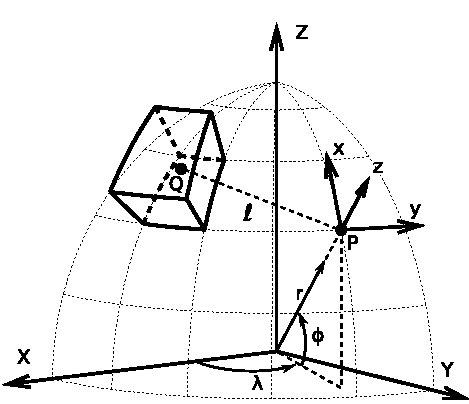
\includegraphics[width=0.9\linewidth]{figures/tesseroid-uieda.pdf}
\caption{
    A spherical prism, also known as  Tesseroid, in a geocentric spherical 
    coordinate system, with a computation point $P$ and its local north 
    oriented Cartesian coordinate system. Picture made by \citet{Uieda2015}.
}
\label{fig:tesseroid-uieda}
\end{figure}

\citet{Uieda2016} developed a forward gravitational model based on 
tesseroids with homogeneous densities using the GLQ approximation 
method.
The main issue of the GLQ is that the approximation becomes less 
accurate when the computation point is closer to the tesseroid of for 
smaler GLQ order \citep{Ku1977}.
Although the model developed by \citet{Uieda2016} uses a second order GLQ, it 
ensures the accuracy implementing a modified version of the adaptive 
discretization of \citet{Li2011}.
It consist in splitting the tesseroid into smaller ones when a certain 
distance-size ratio is lower than a predefined value ($D$) that controls the 
accuracy of the computation.
\citet{Uieda2016} have also objectively obtained standard values of $D$ 
for gravitational potential, gradients and tensor components comparing 
the numerical model with the fields generated by a spherical shell, 
which constitutes a special case of the volume integrals that has 
analytical solution \citep{LaFehr1991, Mikuska2006, Grombein2013} 
\todo[inline]{citar mas??}.

On the other hand, a varying density inside an arbitrary tesseroid 
introduces a new kind of error into the numerical approximation.
This encouraged us to develop a new density-based discretization 
algorithm that divides the tesseroid into smaller ones taking into 
account the variation of the density function.
The number of subdivisions and thus the accuracy of the approximation 
will be controlled by predefined delta ratio $\delta$.

In summary, we present a new forward gravitational model that allows to 
compute the gravitational fields generated by any tesseroid with an 
arbitrary continuous density function on any external point.
It is based on the GLQ approximation whose accuracy is controlled by 
the modified distance-size discretization \citep{Uieda2016} 
and the new density-based discretization algorithms.

In order to ensure the accuracy of the numerical approximation we have 
determined predefined values for the $D$ and $\delta$ parameters by 
comparing the numerical approximation with the analytical solutions for 
a spherical shell with linear and exponential density, which had to be 
derived.

Furthermore, we developed a Python library that implements this forward 
model.
I makes use of some previously existing classes and functions 
from the Python library Fatiando a Terra for geophysical modelling, 
what saved us time and allowed us to focus on the new model.

Furthermore, we have the intention to include it into a future release 
of the Fatiando a Terra library in order to make its distribution and 
maintenance easier.
\todo[inline]{include this?}

In the following sections we will describe how the new algorithm works, its 
theoretical background and obtain default distance-size ratio and delta ratio 
values needed to get an acceptable accuracy in the numerical approximation.

%%%%%%%%%%%%%%%%%%%%%%%%%%%%%%%%%%%%%%%%%%%%%%%%%%%%%%%%%%%%%%%%%%%%%%%%%%%%%%

\section{Theory}

The spherical prisms known as tesseroids are mass elements defined in a 
geocentric spherical coordinate system bounded by a pair of parallels, 
a pair of  meridians, and two concentric spherical surfaces.
We define an external computation point $P(r, \phi, \lambda)$ where the 
gravitational fields generated by the tesseroid are going to be calculated 
with respect to the local north oriented Cartesian coordinate system 
located at $P$.
In the special case of homogeneous density, the gravity potential, its 
gradient and the Marussi tensor components can be calculated through 
the integrals obtained by \citet{Grombein2013} \citep[for same notation 
as the one we will use, see][]{Uieda2016}.

In our case, we will assume that the tesseroid has an arbitrary 
variable density in depth, i.e. only depends on the radial spherical 
coordinate.
Thus, the integrals for the gravitational fields are slightly modified:

\begin{equation}
    V(r,\phi,\lambda) = G
    \int\limits_{\lambda_1}^{\lambda_2}
    \int\limits_{\phi_1}^{\phi_2}
    \int\limits_{r_1}^{r_2}
    \frac{\rho(r')}{\ell} \kappa \,  dr' d\phi' d\lambda',
\label{eq:tesseroid-pot}
\end{equation}
\begin{equation}
    g_{\alpha}(r,\phi,\lambda) = G
    \int\limits_{\lambda_1}^{\lambda_2}
    \int\limits_{\phi_1}^{\phi_2}
    \int\limits_{r_1}^{r_2}
    \rho(r') \frac{\Delta_\alpha}{\ell^3}
    \kappa \, dr' d\phi' d\lambda',
\label{eq:tesseroid-grav}
\end{equation}
\begin{equation}
    g_{\alpha\beta}(r,\phi,\lambda) = G
    \int\limits_{\lambda_1}^{\lambda_2}
    \int\limits_{\phi_1}^{\phi_2}
    \int\limits_{r_1}^{r_2}
    \rho(r') I_{\alpha\beta} \, \kappa \, dr' d\phi' d\lambda' ,
    \label{eq:tesseroid-tensor}
\end{equation}

\noindent where

\begin{equation}
    I_{\alpha\beta} =
    \left(
        \frac{3\Delta_{\alpha} \Delta_{\beta}}{\ell^5} -
        \frac{\delta_{\alpha\beta}}{\ell^3}
    \right) ,
    \label{eq:tesseroid-tensor-kernel}
\end{equation}

\noindent $\alpha, \beta \in \{x, y, z\}$, $\rho(r')$ is the density 
function that depends on the radial coordinate, $\delta_{\alpha\beta}$ 
is Kronecker's delta, $G = 6.674\times10^{-11}\, 
\text{m$^3$kg$^{-1}$s$^{-1}$}$ is the gravitational constant and

\begin{equation}
    \Delta_x = r'[\cos\phi\sin\phi' - \sin\phi\cos\phi'
               \cos(\lambda' - \lambda)],
\end{equation}
\begin{equation}
    \Delta_y = r' \cos \phi' \sin(\lambda' - \lambda),
\end{equation}
\begin{equation}
    \Delta_z = r' \cos \psi - r,
\end{equation}
\begin{equation}
    \kappa = {r'}^2 \cos \phi',
\end{equation}
\begin{equation}
    \ell = \sqrt{{r'}^2 + r^2 - 2 r r' \cos \psi},
\label{eq:ell}
\end{equation}
\begin{equation}
    \cos\psi = \sin\phi\sin\phi' + \cos\phi\cos\phi'
                 \cos(\lambda' - \lambda).
\label{eq:cospsi}
\end{equation}


According to \citet[p.~390]{Hildebrand1987}, we can approximate any 
integral in the interval $[-1, 1]$ using a $N$th order GLQ, i.e. by a 
weighted sum of the integration kernel evaluated on the roots of the 
$N$th Legendre polynomial:

\begin{equation}
    \int\limits_{-1}^1 f(x) dx \approx \sum_{i=1}^N W_i f(x_i),
\end{equation}

\noindent where $x_i$ are the roots of the $N$th Legendre polynomial 
$P_N(x)$ and $W_i$ are the weights of each term:

\begin{equation}
    W_i = \frac{2}{(1-x_i^2)[P_N^\prime(x_i)]^2},
\end{equation}

\begin{equation}
    P_N(x_i) = 0, \quad \forall i = {1,\dots,N}.
\end{equation}

In case of an integration defined on a arbitrary interval, e.g. 
$[a,b]$, we can scale the nodes and perform a similar approximation:

\begin{equation}
    \int\limits_a^b f(x) dx \approx \frac{b-a}{2} \sum_{i=1}^N W_i f(x_i^s),
\label{eq:glq-scaled}
\end{equation}

\noindent where $x_i^s$ is the scaled $x_i$ root into the $[a,b]$ 
interval, also called nodes of the quadrature:

\begin{equation}
    x_i^s = \frac{b-a}{2} x_i + \frac{b+a}{2}.
\end{equation}

\noindent For example, if we use a second order GLQ, the roots of the 
$P_2(x)$ Legendre polynomial and its corresponding weights are $x_i = 
\pm 0.577350269$ and $W_i = 1$.

Our intention is to use GLQ to approximate the volume integrals from 
equations \ref{eq:tesseroid-pot}-\ref{eq:tesseroid-tensor}.
When tesseroids have variable densities, we can write the integral 
kernels as the product of a certain function $g$ and the density 
function:

\begin{equation}
    f(r', \phi', \lambda') = \rho(r') g(r', \phi', \lambda'),
\end{equation}

\noindent and then apply the quadrature to every integral corresponding 
to each spherical coordinate, obtaining a similar expression to the one 
shown by \citet{Asgharzadeh2007} and \citet{Uieda2016}:

\iftwocol{
\begin{equation}
    \begin{split}
        \iiint\limits_\Omega \rho(r') g(r', \phi', \lambda') 
        d\Omega \approx& \\
        A 
        \sum\limits_{i=1}^{N^r}
        \sum\limits_{j=1}^{N^\phi}
        \sum\limits_{k=1}^{N^\lambda}
        & W_i^r W_j^\phi W_k^\lambda \rho(r_i) g(r_i, \phi_j, \lambda_k),
    \end{split}
\label{eq:glq-var-dens}
\end{equation}
}{
\begin{equation}
    \iiint\limits_\Omega \rho(r') g(r', \phi', \lambda') d\Omega \approx
    A 
    \sum\limits_{i=1}^{N^r}
    \sum\limits_{j=1}^{N^\phi}
    \sum\limits_{k=1}^{N^\lambda}
    W_i^r W_j^\phi W_k^\lambda \rho(r_i) g(r_i, \phi_j, \lambda_k),
\label{eq:glq-var-dens}
\end{equation}
}

\noindent where

\begin{equation}
    A = 
    \frac{(\lambda_2 - \lambda_1)(\phi_2 - \phi_1)(r_2 - r_1)}{8}.
\end{equation}

From equation \ref{eq:glq-var-dens} we can observe that the GLQ 
approximates the gravitational fields of a tesseroid as the ones 
generated by $N_\lambda N_\phi N_r$ point masses located at the nodes 
of the Legendre polynomials, where $N_i$ are the orders of the 
quadrature for each integration, with $i \in \{ \lambda, \phi, r \}$, 
in the same way as the GLQ works in the homogeneous density case.
Nevertheless, in this new variable density scenario, the information of 
the density function is summarised into the weights by taking into 
account only the values it assumes on those nodes.
Although this may sound discouraging, we intent to prove otherwise and 
show that this method, along with well suited discretization 
algorithms, approximates the gravitational fields with good accuracy.
\todo[inline]{no se si poner esta ultima oracion}

%%%%%%%%%%%%%%%%%%%%%%%%%%%%%%%%%%%%%%%%%%%%%%%%%%%%%%%%%%%%%%%%%%%%%%%%%%%%%%

\section{Methodology}

From equation \ref{eq:glq-var-dens} we can conclude that the error of 
the numerical approximation is controlled by the order of the 
quadrature, i.e. the number of point masses that are going to be used 
to compute the gravitational field.
This conclusion could lead to a naive methodology: find the order of 
the quadrature that produces gravitational fields with an acceptable 
accuracy.
Although this simple proposal has a few problems: (a) it won't be 
efficient and (b) it couldn't be applied to the general case (any
tesseroid with arbitrary density function on any computational point) 
without modifying the quadrature order taking into account 
characteristics of the tesseroid and the computation point (tesseroid 
size, distance to the computation point, variation of the density 
function, etc).

That's why we will keep the GLQ order fixed and make use of 
discretization algorithms.
Instead of uniformly increase the number of point masses that 
approximates a certain tesseroid, the discretization algorithms are 
intended to efficiently subdivide the tesseroid into smaller ones and 
apply the GLQ to each one of them.
These algorithms generally involve a discretization inequation that 
controls if the tesseroid should be subdivided or not and a certain 
predefined parameter that works as a threshold for the discretization 
inequation.

On the variable density tesseroid problem we found two main error 
sources in the GLQ that should be addressed: (a) the relation between 
the tesseroid size and its distance to the computation point, and (b) 
the variation of the density function.

The former one is also present in the homogeneous density tesseroid 
models, such as the one developed by \citet{Uieda2016}, and could be 
solved by applying a modified version of the adaptive discretization 
algorithm proposed by \citet{Li2011}.
Although for the latter we need to introduce a new density-based 
discretization algorithm that subdivides the tesseroid taking into 
account the variation of its density function.


\subsection{Modified Adaptive Discretization Algorithm}

From equation \ref{eq:glq-var-dens} we saw that the GLQ approximates 
the volume integrals as the gravitational effect of point masses 
located at the nodes of the quadrature. If we set the GLQ orders to 
fixed values, it's easy to conclude that the nearer the computation 
point is to the tesseroid, the accuracy of the approximation is reduced 
and the point masses effect becomes more noticeable than the tesseroid 
we want to approximate. A complete analysis of this conclusion can be 
found in \citet{Ku1977, Li2011, Uieda2016}.

Studying the homogeneous density tesseroid problem, \citet{Ku1977} 
noticed that keeping the GLQ orders fixed, the approximation 
becomes less accurate when the computation point is closer to the 
tesseroid, making the point masses effect more noticeable than the 
tesseroid we want to approximate.
A complete analysis of this conclusion can be found in \citet{Ku1977, 
Li2011, Uieda2016}.

Instead of increasing the GLQ orders to improve the accuracy, what 
leads to a more time consuming computation, \citet{Li2011} proposed an 
adaptive discretization algorithm which essentially consists in 
dividing the tesseroid based on a ratio between the distance to the 
computation point and its dimensions.
\citet{Uieda2016} proposed a modified version of the algorithm proposed 
by \citet{Li2011}. These modifications can be summed up in:
(1) a faster calculation of the distance from the computation point to 
the tesseroid and 
(2) the application of a stack based algorithm that speeds up the 
computation and gives more control over the recursion step.
More specifically, \citet{Uieda2016} redefined the dimensions of an 
arbitrary tesseroid: $L_\lambda$, $L_\phi$ and $L_r$. The former ones 
are the arc-distances measured along its top surface while $L_r$ is the 
difference between the radii of the top and bottom surfaces.

While keeping the GLQ fixed on second orders, the adaptive 
discretization algorithm starts by checking that the following 
inequality is satisfied:

\begin{equation}
    \frac{d}{L_i} \geq D,
\label{eq:distance-size-ratio}
\end{equation}

\noindent where $i \in \{\lambda, \phi, r\}$, $d$ is the distance 
between the geometric centre of the tesseroid and the computation 
point, and $D$ is a predefined value called distance-size ratio.
If the inequality \ref{eq:distance-size-ratio} is not held for at least 
one spherical coordinate, then the tesseroid must be divided by half in 
that direction.
On the contrary, if the inequality is satisfied for every spherical 
coordinate, the algorithm computes the desired gravitational field using the 
GLQ approximation.
A complete description of the modified adaptive discretization 
algorithm can be found in \citet{Uieda2016}.

In summary, the distance-size ratio $D$ determines indirectly how many 
times the tesseroids will be divided, and therefore efficiently 
regulates both the accuracy of the algorithm and its computation time.
Moreover, it limits the computation time by stopping the division of 
the tesseroids when their dimensions are lower than a certain value 
(1mm), assuming that such small tesseroids do not modifies 
significantly the desired gravitational field.

On the other hand, the value assigned to the distance-size ratio $D$ 
cannot be easily related to the error of the approximation, thus the 
choice of the value of $D$ to get an acceptable accuracy must be 
empirically determined beforehand.
In order to overcome this, \citet{Uieda2016} compared the numerical 
computation with the analytical solution for a spherical shell with 
homogeneous density.

We will perform similar tests, but now with variable density spherical 
shell.
From the infinite density functions that can be proposed, we have 
chosen three characteristic ones: a linear, an exponential and a 
discontinuous function.
\todo[inline]{sacaria todo este parrafo y lo introduciria mas adelante}


\subsection{Density-based Discretization Algorithm}

High variations in the density function of an arbitrary tesseroid 
introduces a new type of error into the numerical approximation: only a 
few point masses would not reproduce the effect of this kind of 
variations.
The modified version of the adaptive discretization algorithm may help 
in reducing this kind of error, but as it only takes into account the 
dimensions of the tesseroid and the distance to the computation point, 
it's not well suited to fully perform this task.

In order to overcome this, we developed a complementary discretization 
algorithm that takes into account the variation of the density inside 
the tesseroid. Basically, it subdivides any tesseroid on the radial 
direction on the depth at which the \emph{maximum density variation} 
takes place.

\begin{figure*}
\centering
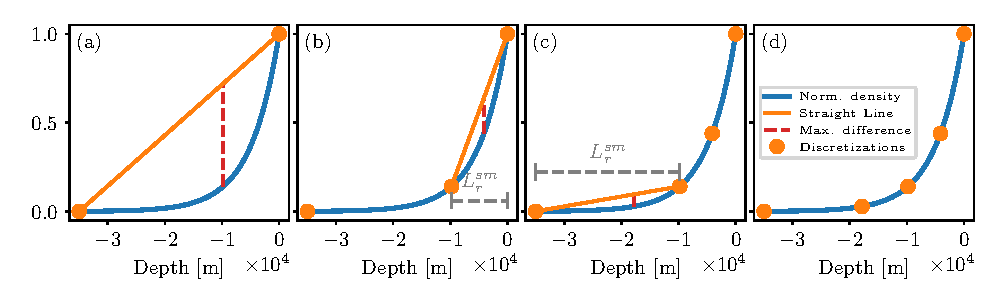
\includegraphics[width=\linewidth]
    {figures/density-based-discretization-algorithm.pdf}
\caption{
    Example intended to show how the density-based algorithm works.}
\label{fig:density-discretization-algorithm}
\end{figure*}

In a general way, the algorithm can be summarised in the following steps:

\begin{enumerate}
\renewcommand{\theenumi}{(\arabic{enumi})}
    \item Normalise the density function to the [0, 1] interval,
    \item Compute the absolute difference between the normalised 
          density and a linear function that assumes the same values on the 
          top and bottom radii that this normalised density.
    \item If product of the maximum of the absolute difference and a 
          tesseroid size ratio is greater that a predefined delta ratio 
          ($\delta$), then the tesseroid will be subdivided on the 
          radius at which this maximum takes place. Otherwise, the 
          tesseroid won't be split.
    \item If it's discretized, then apply items (2), (3) and (4) for 
          every subdividing tesseroid.
\end{enumerate}

Lets assume an arbitrary \emph{original} tesseroid with boundary radii 
$R_1$ and $R_2$ and a density function $\rho(r')$, whose radial 
dimension can be written as $L_r = R_2 - R_1$.

First we need to normalise the density function such as its minimum and 
maximum will be 0 and 1, respectively.
We call this normalised density $\rho_n(r')$ and we calculate it as 
follows:

\begin{equation}
    \rho_n(r') = \frac{\rho(r') - \rho_1}{\rho_2 - \rho_1},
\end{equation}
\noindent where
\begin{equation}
    \rho_1 = \text{min}\{ \rho(r') \}, \quad
    \rho_2 = \text{max}\{ \rho(r') \} \quad
    \forall \, r' \in [R_1, R_2].
\end{equation}

Because the algorithm will be iteratively applied for every 
subdividing tesseroid, we'd like to note that this normalised density 
function will be the same for every subdividing tesseroid.
In case that the density function is constant, both the maximum and 
minimum densities are equal and the normalised function could not 
be defined, so the density-based discretization algorithm won't be 
applied.

Secondly, we must define a linear function $\rho_l(r')$ that assumes 
the same values as the normalised density $\rho_n(r')$ on the boundary 
radii $R_1$ and $R_2$:

\begin{equation}
    \rho_l(r') =
    \frac{ \rho_n(R_2) - \rho_n(R_1) }{ R_2 - R_1 } (r' - R_1) + \rho_n(R_1),
    \label{eq:density-reference-line}
\end{equation}

\noindent and compute the absolute difference between this linear 
function and the normalised density:

\begin{equation}
    \Delta \rho (r') = | \rho_n(r') - \rho_l(r') |.
    \label{eq:density-abs-diff}
\end{equation}

Finally, if the product of the maximum of the absolute difference and a 
tesseroid size ratio is greater than a predefined delta ratio $\delta$ 
we will divide the tesseroid on the radius at which this maximum takes 
place ($R_\text{max}$):

\begin{equation}
    \text{max}\{ \Delta \rho(r') \} \frac{L_r^\text{sm}}{L_r} > \delta,
    \label{eq:delta-density}
\end{equation}

\noindent obtaining a pair of smaller tesseroids with the same 
longitude and latitude boundaries.

The $L_r^\text{sm}$ is the radial dimension of the tesseroid that is 
currently analysed. On the first iteration, this tesseroid is the 
\emph{original} one, so $L_r^\text{sm} = L_r$, but for future 
iterations this radial dimension will be computed as the difference of 
the top and bottom radii of the subdividing tesseroid.

This algorithm will be subsequently applied to every subdividing 
tesseroid.
We will start from equation \ref{eq:density-reference-line} defining a 
new linear function $\rho_l(r')$, an absolute difference with equation 
\ref{eq:density-abs-diff} and evaluate the discretization inequation 
\ref{eq:delta-density}, taking into account that now $R_1$ and $R_2$ 
are the radial boundaries of this smaller tesseroid.

The tesseroid size ratio included in the inequation 
\ref{eq:delta-density} is intended to reduce the number of probable 
unneeded discretizations and focus on discretizations that will 
significantly reduce the numerical error.
A big subdividing tesseroid with small maximum absolute difference would 
introduce more numerical error than a small subdividing tesseroid with 
higher maximum absolute difference.

If on the contrary the inequation \ref{eq:delta-density} is not held, 
then the tesseroid will not be subdivided.
The same happens if the tesseroid radial dimension is bellow the 
threshold of 1mm. On the first case due to the fact that no more 
discretizations are needed, and on the second one because smaller 
tesseroids will not introduce meaningful increases in the accuracy of 
the computation.
This two conditions guarantee that the algorithm is finite.
Once they are met, every subdividing tesseroid is subjected to the 
modified adaptive discretization algorithm and the GLQ in order to 
compute the gravitational field generated by it.

On Figure \ref{fig:density-discretization-algorithm}(a) we propose an 
arbitrary normalised density function as an example of how this 
algorithm works.
And we plotted its corresponding linear function $\rho_l(r')$ and a 
dashed line that represents the maximum absolute difference $\Delta 
\rho (r')$.
We will assume that the discretization inequation 
\ref{eq:delta-density} holds in this case, so we must divide the 
tesseroid at the height at which the maximum difference occurs.
The dots on Figure \ref{fig:density-discretization-algorithm} 
represent the discretization heights, i.e. the radial boundaries of the 
subdividing tesseroids produced by the algorithm.

On Figure \ref{fig:density-discretization-algorithm}(b) we apply the 
algorithm on the shallower subdividing tesseroid.
In the same way, we propose the linear function and compute the maximum 
absolute difference $\Delta \rho (r')$.
In this case, the tesseroid size-ratio $L_r^\text{sm}/L_r$ is lower 
than one and will be taken into account in the discretization 
inequation, which will be assumed to hold also in this case, leading to 
the division of this tesseroid.

On Figure \ref{fig:density-discretization-algorithm}(c) we perform the 
same analysis on the deeper subdividing tesseroid, and assuming that the 
inequality holds in this case we also subdivide it.

Finally, if we suppose that the value of $\delta$ used in this example 
does not produce further discretizations, the resulting subdividing 
tesseroids can be seen on Figure 
\ref{fig:density-discretization-algorithm}(d).

It's easy to see that the delta ratio indirectly controls how many 
times the tesseroids will be subdivided based on the variation of the 
density function.
Therefore it determines the accuracy involving the numerical error that 
the density variation introduces and also the computation time.
This raises the need to determine a maximum value of $\delta$ that 
ensures an acceptable accuracy while minimising the computation time. 
We will perform this determination with the same methodology as the one 
applied to the $D$ ratio: compare the numerical model with the 
analytical solutions for a spherical shell.


\subsection{Algorithm summary}

When computing any gravitational field generated by an arbitrary tesseroid on 
a specific computation point, we present the following methodology:

\begin{enumerate}
    \renewcommand{\theenumi}{(\arabic{enumi})}
    \item Apply the density-based discretization algorithm in case of 
          variable density producing subdivisions of the original tesseroid,
    \item Apply the modified adaptive discretization algorithm for 
          each subdivision, generating a set of smaller tesseroids,
    \item Compute the desired gravitational field for every small tesseroid 
          through the GLQ approximation with fixed quadrature orders
          (equation \ref{eq:glq-var-dens}).
\end{enumerate}

In most practical cases, the forward model will consist in a set of 
tesseroids whose gravitational effect will be computed on a set of 
computation points.
These steps can be applied on every tesseroid and for each computation point,
adding the contribution of each tesseroid to the resulting 
gravitational field.


%%%%%%%%%%%%%%%%%%%%%%%%%%%%%%%%%%%%%%%%%%%%%%%%%%%%%%%%%%%%%%%%%%%%%%%%%%%%%

\section{Determination of distance-size and delta ratios}

In order to determine default values for the distance-size ratio ($D$)
and the delta ratio ($\delta$) that ensure both numerical accuracy and 
computation effectiveness we need to compare the numerical 
approximation with some analytical solutions.

On the homogeneous density tesseroids case, \citet{Uieda2016} and 
\citet{Grombein2013} compared their numerical model with the analytical 
solution of a spherical shell.
We could follow this idea, but for our needs the spherical shell must 
have the same density function as the numerical model, although the 
analytical solution in this case must be derived.


\subsection{Analytical Solutions for Spherical Shell}

The integrals that define the gravity fields in equations 
\ref{eq:tesseroid-pot}-\ref{eq:tesseroid-tensor} have analytical 
solutions in case of a spherical shell with homogeneous density 
\citep{Mikuska2006,Grombein2013}.
But for variable density spherical shell the problem wasn't address in 
the literature yet.

Lets consider a spherical shell with inner and outer radii $R_1$ and 
$R_2$, respectively, whose density depends on the radial spherical 
coordinate (Figure \ref{fig:spherical-shell}).
The gravity potential generated by the shell on an arbitrary external 
point $Q(0,0,r)$, located along the $z$ axe at a distance $r$ from the 
origin, can be written as follows:

\begin{figure}
\centering
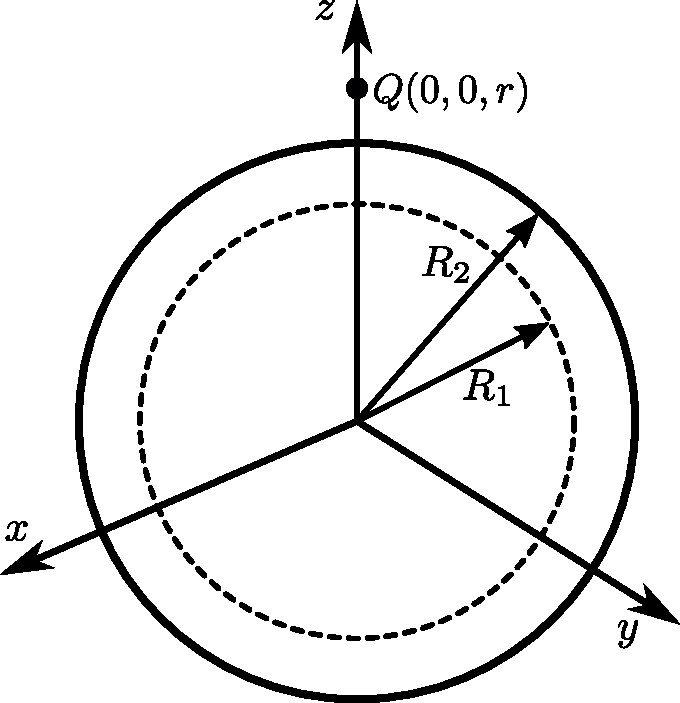
\includegraphics[width=0.7\linewidth]{figures/spherical-shell.pdf}
\caption{
    Spherical shell with inner and outer radii $R_1$ and $R_2$, respectively.
    The computation point $Q$ is located on the $z$ axe at a distance $r$ from
    the centre of the shell.
    For our purposes we will assume that $Q$ is outside the outer radii,
    i.e. $r > R_2$.
    }
\label{fig:spherical-shell}
\end{figure}

\begin{equation}
    V_\text{sh}(r) = G 
    \int\limits_0^{2\pi}
    \int\limits_{-\frac{\pi}{2}}^\frac{\pi}{2}
    \int\limits_{R_1}^{R_2}
    \frac{\rho(r')}{\ell} {r'}^2 \cos\phi' \, 
    dr' d\phi' d\lambda',
\end{equation}

\noindent where $\ell$ is defined in equation \ref{eq:ell}.
The computation point $Q$ is located at latitude $\phi=90^\circ$, so 
$\ell$ and $\cos\psi$ (defined in equation \ref{eq:cospsi}) get 
simplified:

\begin{equation}
    \cos\psi = \sin\phi', \quad
    \ell = \sqrt{r'^2 + r^2 - 2 r r' \sin\phi'}.
\end{equation}

Due to the rotational symmetry along the $z$ axe, the integration in 
$\lambda'$ is straightforward:

\begin{equation}
    V_\text{sh}(r) = 2\pi G 
    \int\limits_{-\frac{\pi}{2}}^\frac{\pi}{2}
    \int\limits_{R_1}^{R_2}
    \frac{\rho(r') {r'}^2 \cos\phi'}{\sqrt{r'^2 + r^2 - 2 r r' \sin\phi'}}
    \, dr' d\phi',
\end{equation}

\noindent while the integration in $\phi'$ can be performed 
independently of the density function.
Making use of SymPy \citep{sympy2017}, a Python library for symbolic 
mathematics, we obtained the following expression for the potential:

\iftwocol{
\begin{equation}
    \begin{split}
        V_\text{sh}(r) = 2\pi G
        \int\limits_{R_1}^{R_2}
        \Big[ & \sqrt{r^2 + r'^2 + 2rr'} - \\
        & \sqrt{r^2 + r'^2 - 2rr'}
        \Big] \frac{r'\rho(r')}{r} \, dr'.
    \end{split}
\label{eq:shell-pot-sqrts}
\end{equation}
}{
\begin{equation}
    V_\text{sh}(r) = 2\pi G
    \int\limits_{R_1}^{R_2}
    \Big[ \sqrt{r^2 + r'^2 + 2rr'}  -
    \sqrt{r^2 + r'^2 - 2rr'} 
    \Big] \frac{r'\rho(r')}{r} \, dr'.
\label{eq:shell-pot-sqrts}
\end{equation}
}

For our purposes we can assume that the computation point $Q$ is 
farther from the origin than the outer radius, i.e. $r>R_2$. 
And taking into account that $r'$ is always lower than $R_2$, we can 
simplify the square roots in equation \ref{eq:shell-pot-sqrts}:

\begin{equation}
    \sqrt{r^2 + r'^2 + 2rr'} = |r + r'| = r + r',
\end{equation}
\begin{equation}
    \sqrt{r^2 + r'^2 - 2rr'} = |r - r'| = r - r',
\end{equation}

\noindent what leads to the following expression of the potential:

\begin{equation}
    V_\text{sh}(r) = \frac{4\pi G}{r}
    \int\limits_{R_1}^{R_2} {r'}^2 \rho(r') \, dr'.
\label{eq:shell-pot}
\end{equation}

The equation \ref{eq:shell-pot} allows to easily obtain the exact 
gravity potential generated by a spherical shell with a variable 
density in depth on any outside point located on the $z$ axe.
Due to the rotational symmetry along any axe that passes through the 
centre of the shell, the expression in equation \ref{eq:shell-pot} 
reproduces the gravity potential field on any outside point at distance 
$r$ from the its centre.

The gradient and the Marussi tensor derived from potentials that 
depends solely on $r$ have only a few non zero components: the vertical 
component of the gradient ($g_z$) and the diagonal components of the 
tensor ($g_{xx}$, $g_{yy}$, $g_{zz}$).
They can be easily obtained as \citet{Grombein2013} does, even for any 
arbitrary density function $\rho(r')$:

\begin{equation}
    g_z = \frac{V_\text{sh}(r)}{r},
\end{equation}
\begin{equation}
    g_{xx} = g_{yy} = -\frac{V_\text{sh}(r)}{r^2}, \quad
    g_{zz} = \frac{2V_\text{sh}(r)}{r^2}.
\end{equation}

For future purposes we are going to obtain the gravity potential for 
three different functions from the perspective of their variation in 
$r'$: a linear and an exponential density function.
\todo[inline]{lo sacaria}


\subsection{Linear Density}

Lets consider a linear density function like:

\begin{equation}
    \rho(r') = ar' + b.
\end{equation}

\noindent The gravitational potential generated by a spherical shell 
with this density on any external point at distance $r$ from its centre 
can be obtained from the following expression:

\begin{equation}
    V_\text{sh}^\text{lin}(r) = \pi G \left[ 
    a \frac{R_2^4 - R_1^4}{r} +
    b \,\frac{4}{3} \frac{R_2^3 - R_1^3}{r} \right].
    \label{eq:shell-pot-linear}
\end{equation}

\noindent The first term on equation \ref{eq:shell-pot-linear} 
reproduces the potential generated by a spherical shell with variable 
density $\rho(r') = ar'$, while the second one constitutes the 
potential generated by a spherical shell with homogeneous density $\rho 
= b$ \citep{Mikuska2006,Grombein2013}. So the potential can be read as 
the one generated by a combination of both shells.

When applying the density-based discretization algorithm on any 
tesseroid with linear density, the absolute difference defined in 
equation \ref{eq:density-abs-diff} will always be zero, so the 
discretization inequation \ref{eq:delta-density} will never be 
satisfied.
Therefore, independently of the linear function proposed, the 
density-based algorithm will never be applied, leaving the modified 
adaptive discretization algorithm as the only mechanism to control the 
accuracy of the numerical approximation.
That's why we only need to determine the minimum value of $D$ needed in 
order to guarantee an acceptable accuracy while ignoring the value of 
$\delta$.

In order to compare the numerical model with the analytical solution we 
must build a spherical shell from a set of tesseroids.
We propose a mesh of $30^\circ \times 30^\circ$ tesseroids to compute 
the gravitational potential, the vertical component of the gradient 
($g_z$) and the diagonal components of the Marussi tensor ($g_{xx}$, 
$g_{yy}$, $g_{zz}$) on four different grids: (1) a grid located at the 
pole, (2) another one on the Equator, (3) one located at satellite 
height and (4) a big grid of $30^\circ \times 30^\circ$.
More information about this grids can be found on Table 
\ref{tab:grids}.

We have computed these gravitational fields on every point of the four 
grids for different values of $D$, ranging from 0.5 to 10 with a step 
of 0.5.
Then we calculated the maximum difference between these results and the 
value that the analytical solution assumes at the same height.
Because the gravity fields generated by a tesseroid are approximated by 
the effect of point masses, the numerical results may vary between 
computation points at same height but at different latitude or 
longitude.
That's why we choose for comparison the maximum difference between the 
results on every point of the grid and the analytical solution.

Finally, we will set the acceptable value of $D$ as the minimum value 
at which the corresponding error of the numerical approximation is 
lower than 0.1\%.

\begin{table}
\caption{
    Description of the synthetic grids on which the comparison of the 
    numerical model against the analytical solutions for a spherical 
    shell was done.
    This collection of grids tries to include every possible scenario 
    on which the numerical model can present a different behaviour 
    depending on the size of the grid, its location or its height over 
    the Earth surface. Every grid consists in a set of 10$\times$10 
    points.
}
\label{tab:grids}
\begin{tabular}{lcccc}
    Grid & Size & Lat. extension & Lon. extension & Height \\ \hline
    Pole & $1^\circ \times 1^\circ$ & $89^\circ - 90^\circ$ &
        $0^\circ - 1^\circ$ & 2km \\
    Equator & $1^\circ \times 1^\circ$ & $0^\circ - 1^\circ$ &
        $0^\circ - 1^\circ$ & 2km \\
    Satellite & $1^\circ \times 1^\circ$ & $89^\circ - 90^\circ$ &
        $0^\circ - 1^\circ$ & 260km \\
    Big Grid & $30^\circ \times 30^\circ$ & $60^\circ - 90^\circ$ &
        $0^\circ - 30^\circ$ & 2km \\
\end{tabular}
\end{table}

In order to perform the comparison, we proposed a thin and a thick 
spherical shells with 1km and 35km of thickness, respectively, whose 
outer radii is equal to the mean Earth radius.
On both cases we will suppose that the density assumes a value of 
2670~kg/m$^3$ on the outer surface and 3300~kg/m$^3$ at the inner 
radius:

\begin{equation}
    \rho(r') = ar' + c,
    \label{eq:density-linear}
\end{equation}
\noindent with 
\begin{equation}
    a = -\frac{3300\text{kg/m$^3$} - 2670\text{kg/m$^3$}}{R_2 - R_1},
\end{equation}
\begin{equation}
    c = \frac{3300\text{kg/m$^3$} - 
        2670\text{kg/m$^3$}}{R_2 - R_1} R + 
        2670\text{kg/m$^3$},
\end{equation}

\noindent where $R$ = 6378.137 km is the mean Earth radius.

Then we computed the percentage difference between the numerical model 
with its corresponding analytical solution (equation 
\ref{eq:density-linear}) for the thick and the thin spherical shell.

We can see the results for the potential, the vertical component of the 
gradient $g_z$ and the $g_{zz}$ component of the Marussi tensor on 
Figures \ref{fig:D-linear-thin} and \ref{fig:D-linear-thick}.
We exclude the results corresponding to the other two diagonal 
components of the tensor because they are similar to the ones obtained 
for the $g_{zz}$, although they can be found on the repository. 
\todo[inline]{chequear}

For the linear density case, we can observe that the calculation of the 
potential and the $g_z$ component of its gradient needs a value of 
$D=1$ and $D=2$, respectively, in order to ensure an accuracy of 0.1\%.
On the other hand, the $g_{zz}$ computations show a noticeable 
difference between the thin and the thick shell: the first one needs a 
value of $D$ equal to 8 while the later only a $D$ of 3.5.
We will keep the more conservative result of $D$ equal to 8 in case of 
computing the Marussi tensor components in case of a linear density 
tesseroid.

\begin{figure*}
\centering
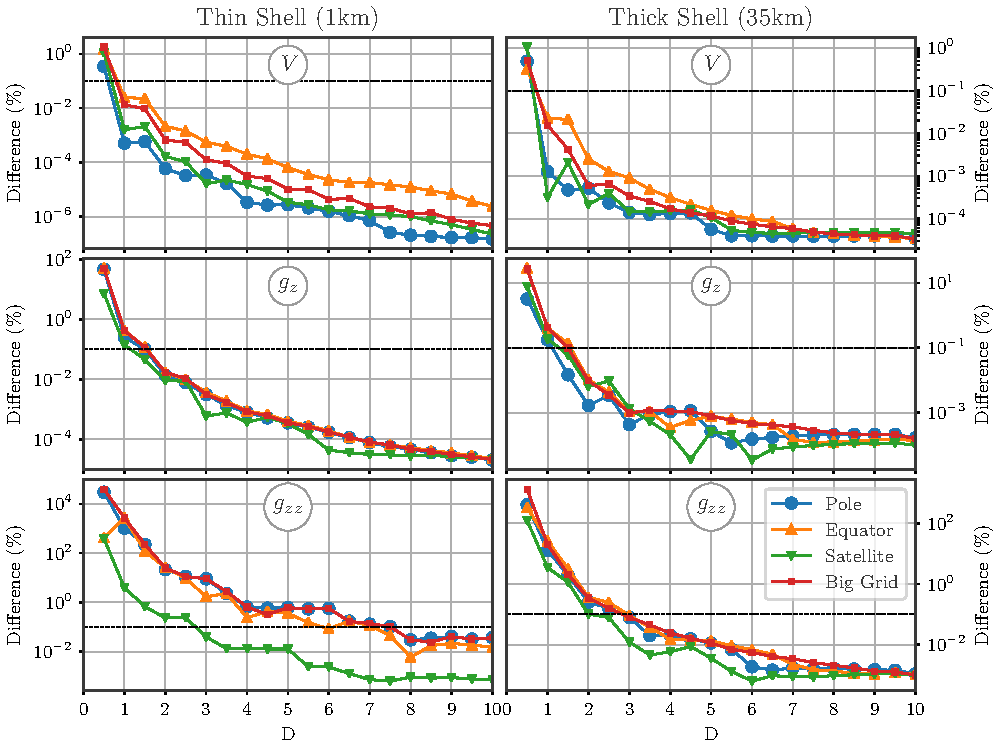
\includegraphics[width=0.9\linewidth]{figures/linear-D.pdf}
\caption{
    Differences between the gravity fields generated by the numerical 
    model and the analytical solution for (a) a thin spherical shell of 
    1km of thickness and (b) a thick spherical shell of 35km of thickness,
    both with the linear density defined on equation 
    \ref{eq:density-linear}.
    The computations were performed on the four grids described in 
    Table \ref{tab:grids}, for different values of the distance-size 
    ratio $D$ and without applying the density-based discretization 
    algorithm.
    If the difference is less than 0.1\%, we consider that the model 
    has achieved an acceptable accuracy for the corresponding value of 
    $D$.
    }
\label{fig:D-linear}
\end{figure*}


\subsection{Exponential Density}

A more complex density variation than a linear one could be an 
exponential function like:

\begin{equation}
    \rho(r') = Ae^{-(r' - \Delta h)/b},
\end{equation}

\noindent where $A$, $\Delta h$ and $b$ are constants.
The gravitational potential field generated by a spherical shell with 
this kind of density function on any external point at a distance $r$ 
from its centre can be calculated as follows:

\iftwocol{
\begin{equation}
    \begin{split}
        V_\text{sh}^\text{exp}(r) = \frac{4\pi G}{r} 
        Ab 
        \Big[
        & (R_1^2 + 2R_1 b + 2b^2)e^{-\frac{R_1 - \Delta h}{b}} - \\
        & (R_2^2 + 2R_2 b + 2b^2)e^{-\frac{R_2 - \Delta h}{b}}
        \Big].
    \end{split}
\label{eq:shell-pot-exp}
\end{equation}
}{
\begin{equation}
    V_\text{sh}^\text{exp}(r) = \frac{4\pi G}{r} 
    Ab \, e^\frac{\Delta h}{b}
    \Big[
    (R_1^2 + 2R_1 b + 2b^2)e^{-\frac{R_1}{b}} - \\
    (R_2^2 + 2R_2 b + 2b^2)e^{-\frac{R_2}{b}}
    \Big].
\label{eq:shell-pot-exp}
\end{equation}
}

This expression will allow us  to perform comparisons between the 
analytical solutions and the numerical approximation, similar as the 
ones made for the linear density case.
Although in the exponential density scenario the problem is more 
complex due to the fact that the density-based discretization must be 
used together with the modified adaptive discretization algorithm.
This means that both the distance-size ratio $D$ and the delta ratio 
$\delta$ must be simultaneously determined.

From every $D$ and $\delta$ combination we want to find the one that 
produces a numerical error lower than the 0.1\% threshold while keeping 
an effective computation, i.e. the ($D$, $\delta)$ pair that produces 
the minimum number of discretizations and ensures an acceptable 
numerical precision.
We can propose an heuristic method to perform this task: compute the 
numerical error for every ($D$, $\delta$) points belonging to a grid on 
the $D$, $\delta$ space and specify the pair that combines an 
acceptable numerical error with an efficient computation.

\begin{figure}
\centering
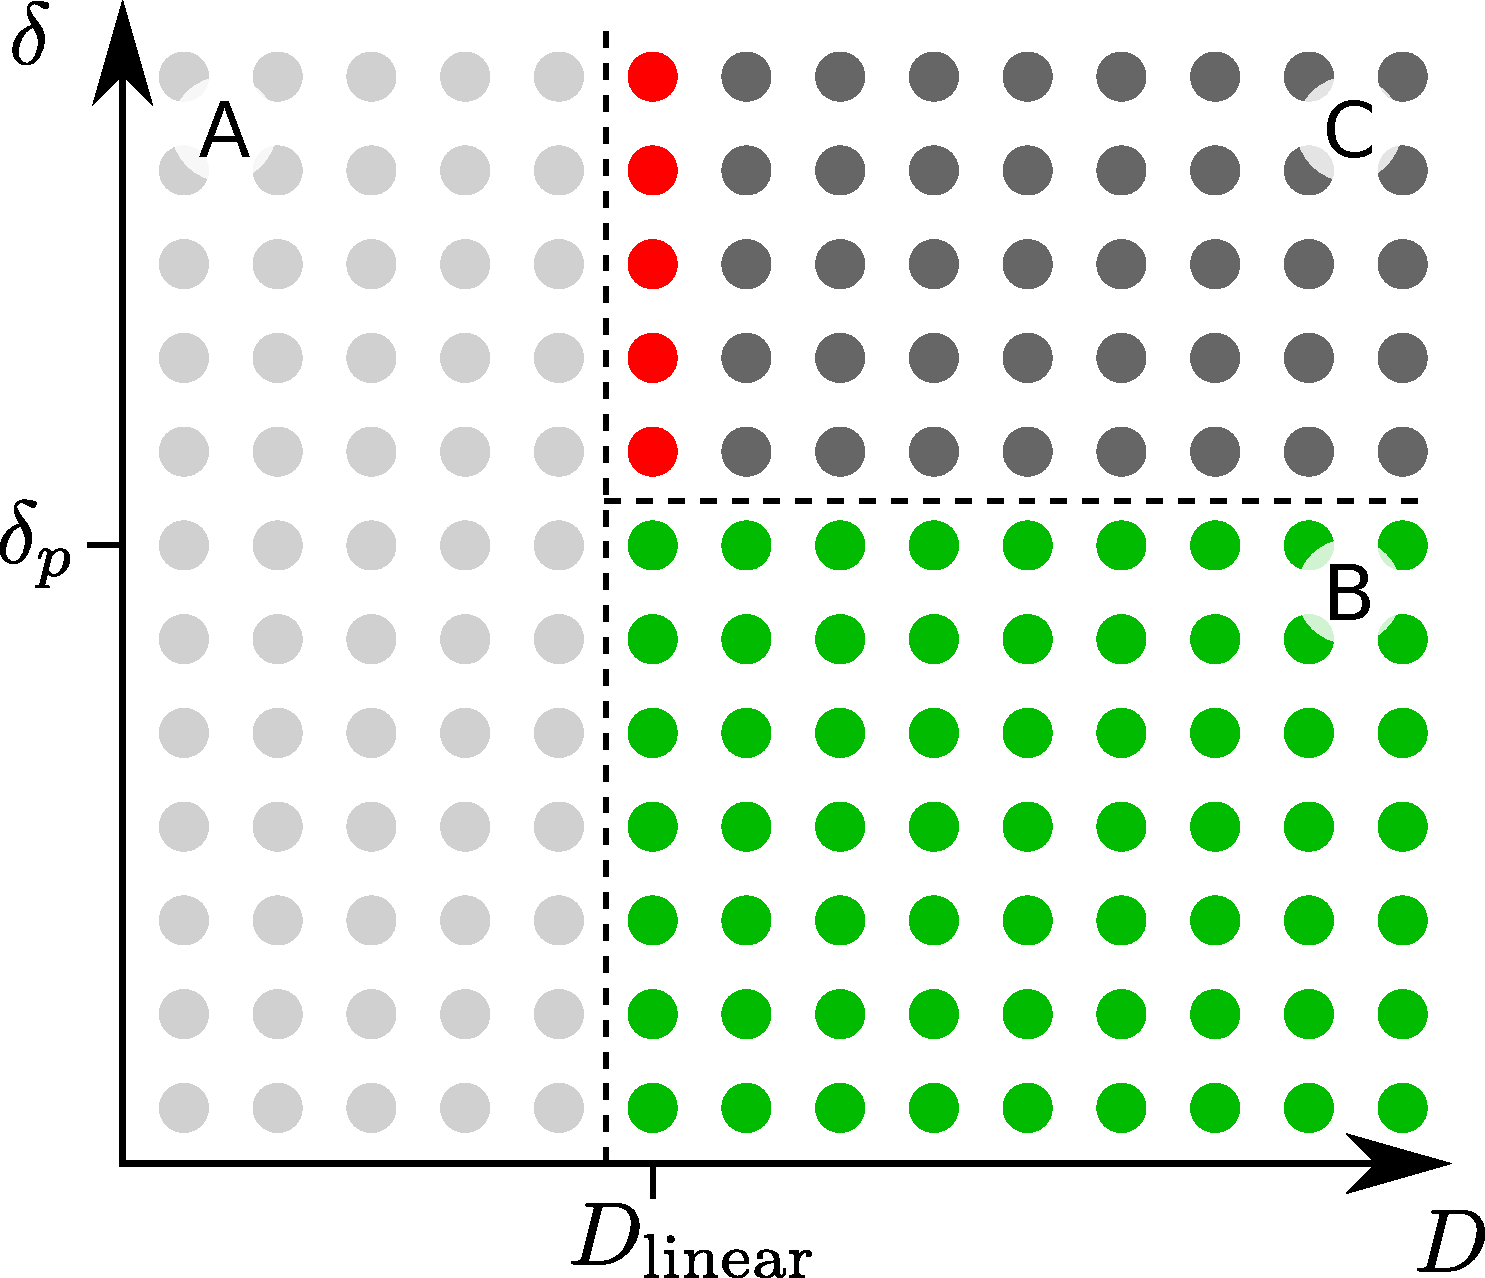
\includegraphics[width=\linewidth]
    {figures/D-delta-grid-search.pdf}
\caption{
    $D$, $\delta$ space divided in three regions (A, B and C) based on 
    the definitions of $D_\text{linear}$ and $\delta_p$ (see text for more 
    information).
    Light grey points are the non-eligible ($D$, $\delta$) pairs 
    belonging to the region A (with $D < D_\text{linear}$).
    Green points have acceptable numerical error (lower than 0.1\%), 
    while the red ones represent those whose error is greater than the 
    threshold.
    Dark grey points represent those from which we don't have a priori 
    information about their numerical error.}
\label{fig:D-delta-grid-search}
\end{figure}

Because the algorithm is intended to work with default $D$ and $\delta$ 
values that ensures these two conditions for every density function, 
the default value for $D$ cannot be lower than the one determined for 
the linear function.
That's why we can only choose the ($D$, $\delta$) points on which
$D \geq D_\text{linear}$.
In this way we can divide the $D$, $\delta$ space in two subregions: 
one with $D < D_\text{linear}$ and other with $D \ge D_\text{linear}$.
We can ignore points belonging to the former one (region A on Figure 
\ref{fig:D-delta-grid-search}) and focus on the latter (regions B and C 
on Figure \ref{fig:D-delta-grid-search}).

From the $D \ge D_\text{linear}$ subregion we can explore the numerical 
error of points with $D = D_\text{linear}$ and different values of 
$\delta$.
We will call $\delta_p$ as the maximum $\delta$ at which the numerical 
error is lower than the 0.1\% threshold while keeping
$D = D_ \text{linear}$.
Greater $\delta$ values than $\delta_p$ will produce computations 
with high error, while lower $\delta$ values than $\delta_p$ will 
produce more discretizations leading to non-efficient computation.

With this definition in mind we can subdivide the subregion in two: one 
with points with $\delta \le \delta_p$ (region B on Figure 
\ref{fig:D-delta-grid-search}) and other with points with $\delta > 
\delta_p$ (region C on Figure \ref{fig:D-delta-grid-search}).

It worth mention that a greater $D$ or a lower $\delta$ 
increases the number of discretizations of the tesseroid.
Although a greater $D$ may divide it in the latitude, longitude 
and/or radial direction; a lower $\delta$ will only discretize the 
original tesseroid in the radial direction.
This means that a decrease in $\delta$ will produce a more efficient 
computation than an increase in $D$.
\todo[inline]{Should we keep this paragraph? The same is explained bellow.}

Every point in the subregion with $\delta \le \delta_p$ (region B on 
Figure \ref{fig:D-delta-grid-search}) will have a numerical error lower 
than the 0.1\% threshold, but they will always produce more 
discretizations than the ($D_\text{linear}$, $\delta_p$) point leading 
to non-efficient computations.

On the other hand, we have no a priori information about the numerical 
error of points with $\delta > \delta_p$ (region C on 
Figure \ref{fig:D-delta-grid-search}).
Although, if we find a point with acceptable numerical error in this 
region, we know it will produce more discretizations than the 
($D_\text{linear}$, $\delta_p$) point, leading to a non-efficient 
computation.
This is due to the fact that even an increase in $\delta$ will produce 
less density-based discretizations, the increase in $D$ will introduce 
even more subdivisions not only in the radial direction, but 
also in the latitude and longitude ones.

In conclusion, the ($D$, $\delta$) point that minimises the number of 
discretizations while keeping an acceptable numerical error under the 
0.1\% threshold is the one on which the ratio $D$ is equal to 
$D_\text{linear}$ and the delta ratio is $\delta_p$.


\todo[inline, color=red]{Text bellow is old}
%%%%%%%%%%%%%%%%%%%%%%%%%%%%%%%%%%%%%%%%%%%%%%%%%%%%%%%%%%%%%%%%%%%%%%%%%%%%%%

\subsubsection{Linear Density}

If the density of the spherical shell is a linear function on the radial coordinate, i.e.:

\begin{equation}
    \rho(r') = ar' + b,
\end{equation}

\noindent then the gravity potential generated on any computation point at distance $r$ from its centre can be obtained from the following expression:

\begin{equation}
    V_\text{sh}^\text{lin}(r) = \pi G \left[ 
    a \frac{R_2^4 - R_1^4}{r} +
    b \,\frac{4}{3} \frac{R_2^3 - R_1^3}{r} \right].
    \label{eq:shell-pot-linear}
\end{equation}

The first term on equation \ref{eq:shell-pot-linear} reproduces the potential generated by a spherical shell with variable density $\rho(r') = ar'$, while the second one constitutes the potential generated by a spherical shell with homogeneous density $\rho = b$ \citep{Mikuska2006,Grombein2013}.
So the potential can be read as the one generated by a combination of both shells.


\subsubsection{Exponential Density}

If, on the other hand, the spherical shell has an exponential density in the radial coordinate,

\begin{equation}
    \rho(r') = Ae^{-(r' - \Delta h)/b},
\end{equation}

\noindent the potential (calculated through SymPy \citep{sympy2017}) can be written as follows:

\iftwocol{
\begin{equation}
    \begin{split}
        V_\text{sh}^\text{exp}(r) = \frac{4\pi G}{r} 
        Ab 
        \Big[
        & (R_1^2 + 2R_1 b + 2b^2)e^{-\frac{R_1 - \Delta h}{b}} - \\
        & (R_2^2 + 2R_2 b + 2b^2)e^{-\frac{R_2 - \Delta h}{b}}
        \Big].
    \end{split}
\label{eq:shell-pot-exp}
\end{equation}
}{
\begin{equation}
    V_\text{sh}^\text{exp}(r) = \frac{4\pi G}{r} 
    Ab \, e^\frac{\Delta h}{b}
    \Big[
    (R_1^2 + 2R_1 b + 2b^2)e^{-\frac{R_1}{b}} - \\
    (R_2^2 + 2R_2 b + 2b^2)e^{-\frac{R_2}{b}}
    \Big].
\label{eq:shell-pot-exp}
\end{equation}
}

%%%%%%%%%%%%%%%%%%%%%%%%%%%%%%%%%%%%%%%%%%%%%%%%%%%%%%%%%%%%%%%%%%%%%%%%%%%%%%%

\section{Implementation}

We have developed a Python library that computes the gravity fields generated by any Tesseroid with variable density in depth.
It is freely available under the BSD 3-clause open-source library and can be downloaded from the following repository: \todo[inline]{agregar repo, vale la pena poner el link?}

This new library approximates the gravitational effect of each tesseroid through the GLQ, and guarantees its accuracy with the modified version of the adaptive discretization algorithm, original developed by \citet{Li2011} and improved by \citet{Uieda2016}, and a new density-based discretization algorithm.
The later one had to be developed in order to decrease a new type of error in the numerical approximation caused by high variations in the density functions.

The new forward model is based on the preexisting code developed by \citet{Uieda2016} (and included in Fatiando a Terra v.0.5, \citet{Uieda2013}) that is able to compute the gravitational effects of tesseroids with homogeneous density.
On that implementation \citet{Uieda2016} have optimised the more time consuming functions through the Numba compiler.
In contrast, we have decided to develop our new library in Cython language due to difficulties when passing a Python function as argument to precompiled Numba methods, keeping the homogeneous tesseroid calculation and adding the new variable density computations.
The Cython language is a superset of Python language that allows to generate efficient C code through the Cython compiler, producing a library whose functions can be called from regular Python code.

Moreover, it is also compatible with the preexisting open-source library Fatiando a Terra and its usage is very similar to the one for homogeneous tesseroids:

\begin{enumerate}
\renewcommand{\theenumi}{(\arabic{enumi})}
    \item Define a single tesseroid (or a set of several tesseroids) with the Fatiando a Terra classes.
    \item Add a predefined Python density function to the tesseroid (or to each tesseroid in the set).
    \item Calculate the desired gravity field (potential, gradient or tensor components) on any set of computation points.
\end{enumerate}




%%%%%%%%%%%%%%%%%%%%%%%%%%%%%%%%%%%%%%%%%%%%%%%%%%%%%%%%%%%%%%%%%%%%%%%%%%%%%%%

\section{Determination of distance-size ratio}

In order to determine the minimum value for the distance-size ratio $D$ such the numerical approximation achieves an acceptable accuracy, we have compared the numerical model with the analytical solutions for a spherical shell with variable density for three special cases: a linear, an exponential and a discontinuous density function.
The first one constitutes the simplest variation, the second one represents a higher varying function, while the later one tries to emulate a contact between two different media (e.g. crust and mantle interface).

We approximated the spherical shell by a mesh of $30^\circ \times 30^\circ$ tesseroids and calculated the gravity potential, the vertical component of the gradient ($g_z$) and the diagonal components of the Marussi tensor ($g_{xx}$, $g_{yy}$, $g_{zz}$) on four different grids: (1) a grid located at the pole, (2) another one on the Equator, (3) one located at satellite height and (4) a big grid of $30^\circ \times 30^\circ$.
More information about this grids can be found on Table \ref{tab:grids}.

We computed these gravity fields on every point of the four grids for different values of $D$, ranging from 0.5 to 10 with a step of 0.5, without applying the density-based discretization algorithm in order to isolate the behaviour of the adaptive discretization one.
Then we calculated the maximum difference between these results and the value that the analytical solution assumes at the same height.

Because the gravity fields generated by a tesseroid are approximated by the effect of point masses, the numerical results may vary between computation points at same height but at different latitude or longitude.
That's why we choose for comparison the maximum difference between the results on every point of the grid and the analytical solution.

Finally, we set the acceptable value of $D$ if the corresponding error of the numerical approximation is lower than 0.1\%.

\begin{table}
\caption{
    Description of the synthetic grids on which the comparison of the numerical model against the analytical solutions for a spherical shell was done. This collection of grids tries to include every possible scenario on which the numerical model can present a different behaviour depending on the size of the grid, its location or its height over the Earth surface. Every grid consists in a set of 10$\times$10 points.
}
\label{tab:grids}
\begin{tabular}{lcccc}
    Grid & Size & Lat. extension & Lon. extension & Height \\ \hline
    Pole & $1^\circ \times 1^\circ$ & $89^\circ - 90^\circ$ & $0^\circ - 1^\circ$ & 2km \\
    Equator & $1^\circ \times 1^\circ$ & $0^\circ - 1^\circ$ & $0^\circ - 1^\circ$ & 2km \\
    Satellite & $1^\circ \times 1^\circ$ & $89^\circ - 90^\circ$ & $0^\circ - 1^\circ$ & 260km \\
    Big Grid & $30^\circ \times 30^\circ$ & $60^\circ - 90^\circ$ & $0^\circ - 30^\circ$ & 2km \\
\end{tabular}
\end{table}


\subsection{Linear Density}
Firstly,  we proposed a spherical shell with linear density in such way it assumes 2670~kg/m$^3$ on the surface of the Earth and 3300~kg/m$^3$ at the inner radius:

\begin{equation}
    \rho(r') = ar' + c,
    \label{eq:density-linear}
\end{equation}
\noindent with 
\begin{equation}
    a = -\frac{3300\text{kg/m$^3$} - 2670\text{kg/m$^3$}}{R_2 - R_1},
\end{equation}
\begin{equation}
    c = \frac{3300\text{kg/m$^3$} - 
        2670\text{kg/m$^3$}}{R_2 - R_1} R + 
        2670\text{kg/m$^3$},
\end{equation}

\noindent where $R$ = 6378.137 km is the mean Earth radius.

Then we computed the difference between the numerical model with its corresponding analytical solution (equation \ref{eq:density-linear}) for a thick and a thin spherical shell of 1km and 35km of thickness, respectively.

We can see the results for the potential, the vertical component of the gradient $g_z$ and the $g_{zz}$ component of the Marussi tensor on Figures \ref{fig:D-linear-thin} and \ref{fig:D-linear-thick}.
We exclude the results corresponding to the other two diagonal components of the tensor because they are similar to the ones obtained for the $g_{zz}$, although they can be found on the repository. \todo[inline]{chequear}

For the linear density case, we can observe that the calculation of the potential and the $g_z$ component of its gradient needs a value of $D=1$ and $D=2$, respectively, in order to ensure an accuracy of 0.1\%.
On the other hand, the $g_{zz}$ computations show a noticeable difference between the thin and the thick shell: the first one needs a value of $D$ equal to 8 while the later only a $D$ of 3.5.
We will keep the more conservative result of $D$ equal to 8 in case of computing the Marussi tensor components in case of a linear density tesseroid.

\begin{figure}
\centering
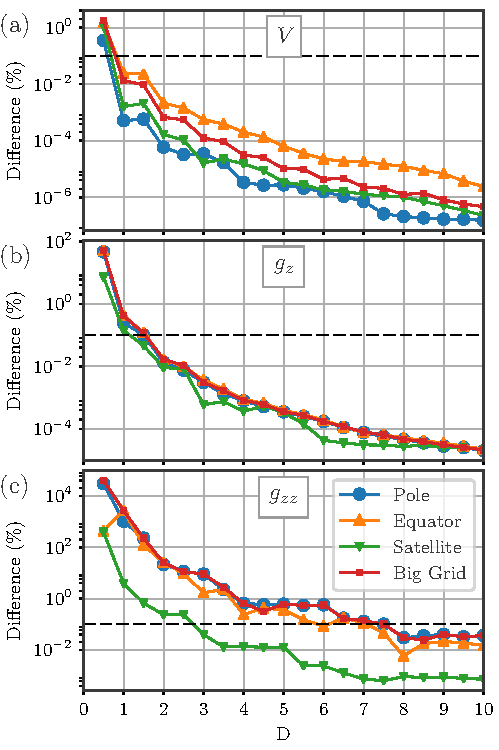
\includegraphics[width=0.9\linewidth]{figures/linear-D-thin.pdf}
\caption{
    Differences between the gravity fields generated by the numerical model and the analytical solution for a thin spherical shell of 1km of thickness with the linear density defined on equation \ref{eq:density-linear}. The computations were performed on the four grids described in Table \ref{tab:grids}, for different values of the distance-size ratio $D$ and without applying the density-based discretization algorithm. If the difference is less than 0.1\%, we consider that the model has achieved an acceptable accuracy for the corresponding value of $D$.
}
\label{fig:D-linear-thin}
\end{figure}

\begin{figure}
\centering
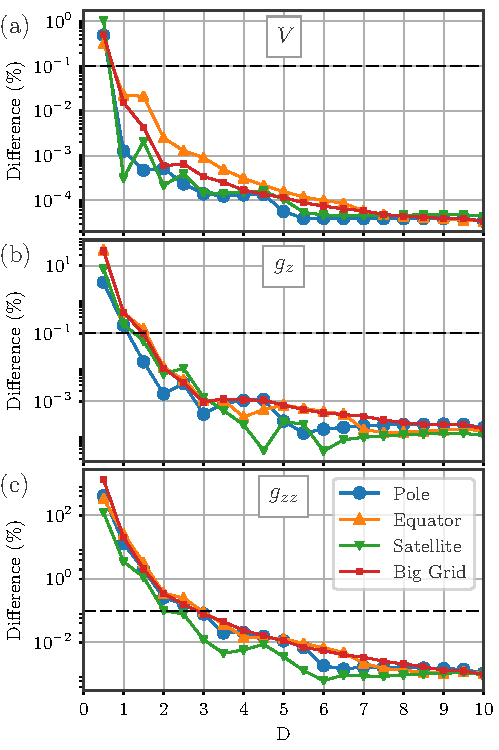
\includegraphics[width=0.9\linewidth]{figures/linear-D-thick.pdf}
\caption{
    Differences between the gravity fields generated by the numerical model and the analytical solution for a thick spherical shell of 35km of thickness with the linear density defined on equation \ref{eq:density-linear}. The computations were performed on the four grids described in Table \ref{tab:grids}, for different values of the distance-size ratio $D$ and without applying the density-based discretization algorithm. If the difference is less than 0.1\%, we consider that the model has achieved an acceptable accuracy for the corresponding value of $D$.
}
\label{fig:D-linear-thick}
\end{figure}


\subsection{Exponential Density}

To test the model in case of an exponential density we proposed the following function:

\begin{equation}
    \rho(r') = A e^{-(r' - R)/b} + C,
\label{eq:density-exp}
\end{equation}
\noindent where
\begin{equation}
    A =
    (3300 \text{kg/m}^3 - 2670 \text{kg/m}^3)
    \left( e^{( R_2 - R_1 )/b} - 1 \right)^{-1},
\end{equation}
\begin{equation}
    C =
    2670 \text{kg/m}^3 - A,
\end{equation}

\noindent and the value of $b$ equal to the thickness of the spherical shell we will use to perform the test.
In this way, the density function assumes the values of 2670 kg/m$^3$ and 3300 kg/m$^3$ on the shell's outer and inner radii, respectively.
The analytical solution of the gravity potential is easily obtained as the sum of the ones for a pure exponential function (like the one in equation \ref{eq:density-exp}) and for an homogeneous spherical shell.

We have performed this test also with a thin and a thick shell of 1 km and 35 km, respectively, without applying the density-based discretization algorithm.
On both cases, the constant $b$ is equal to the thickness of the shell: 1km for the thin shell and 35km for the thick one.
The results can be seen in Figures \ref{fig:D-exp-thin} and \ref{fig:D-exp-thick}.
Once again, we exclude the ones corresponding to $g_{xx}$ and $g_{yy}$ due to their similarity with the ones obtained for $g_{zz}$, although they can be found in the repository.

\begin{figure}
\centering
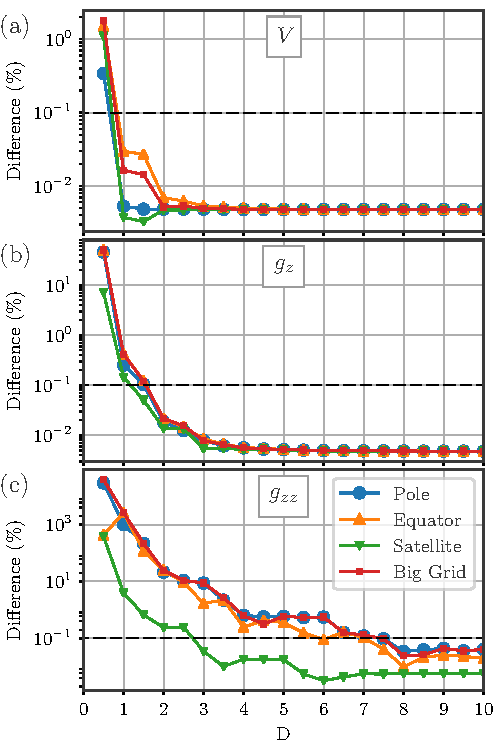
\includegraphics[width=0.9\linewidth]{figures/exponential-D-thin.pdf}
\caption{
    Differences between the gravity fields generated by the numerical model and the analytical solution for a thin spherical shell of 1km of thickness with the exponential density defined on equation \ref{eq:density-exp}. The computations were performed on the four grids described in Table \ref{tab:grids}, for different values of the distance-size ratio $D$ and without applying the density-based discretization algorithm. If the difference is less than 0.1\%, we consider that the model has achieved an acceptable accuracy for the corresponding value of $D$.
}
\label{fig:D-exp-thin}
\end{figure}

\begin{figure}
\centering
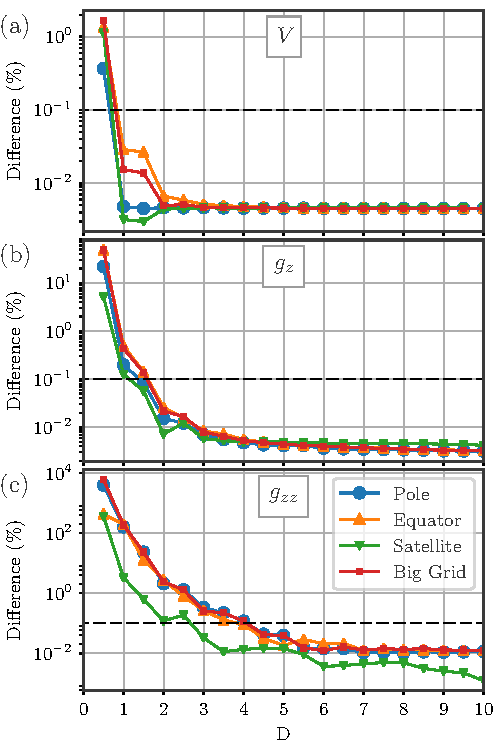
\includegraphics[width=0.9\linewidth]{figures/exponential-D-thick.pdf}
\caption{
    Differences between the gravity fields generated by the numerical model and the analytical solution for a thick spherical shell of 35km of thickness with the exponential density defined on equation \ref{eq:density-exp}. The computations were performed on the four grids described in Table \ref{tab:grids}, for different values of the distance-size ratio $D$ and without applying the density-based discretization algorithm. If the difference is less than 0.1\%, we consider that the model has achieved an acceptable accuracy for the corresponding value of $D$.
}
\label{fig:D-exp-thick}
\end{figure}

In the same way we analysed the linear density results, we can summarise that the thin spherical shell presents the more conservative values of the distance-size ratio: $D=1$ for the gravity potential, $D=2$ for its gradient components and $D=8$ for the Marussi tensor components.

Moreover, we can see that the differences for the potential and the $g_z$ component of the gradient keep constant even for high values of $D$.
Our interpretation is that the modified adaptive discretization algorithm is limited when increasing the accuracy for this density function, supporting the need of a density-based discretization algorithm.

Because the constant $b$ controls the variation of the density function, we wanted to test how does the accuracy of the method behaves at different values of $b$ when the density-based discretization algorithm is not applied.
In order to do this we proposed a thin spherical shell (1km of thickness) with a set of density functions, each one with a different value of $b$.
We computed the difference between the Marussi tensor component $g_{zz}$ generated by the numerical model on the big grid of 30$^\circ\times$30$^\circ$ (see Table \ref{tab:grids}) and the corresponding analytical solution.
These differences were calculated for each proposed density function and for the same set of values of $D$ we have been using on the previous tests, obtaining one curve for each value of $b$.

On Figure \ref{fig:D-exp-power-thin}a we can see the density functions used to perform these tests and its corresponding results on \ref{fig:D-exp-power-thin}b .
Taking into account that lower values of $b$ implies a more varying function, we can see that for high varying functions the numerical model does not perform well: for $b=100$m the difference is almost 100\%.

We can conclude that even when the density-based discretization algorithm is not applied, the numerical approximation performs under the acceptable threshold for values of $b$ greater than the thickness of the shell, i.e. for low density variations.
On the other hand, a density-based discretization algorithm is needed in order to guarantee the accuracy of the approximation in case of a high varying density function.

\begin{figure}
\centering
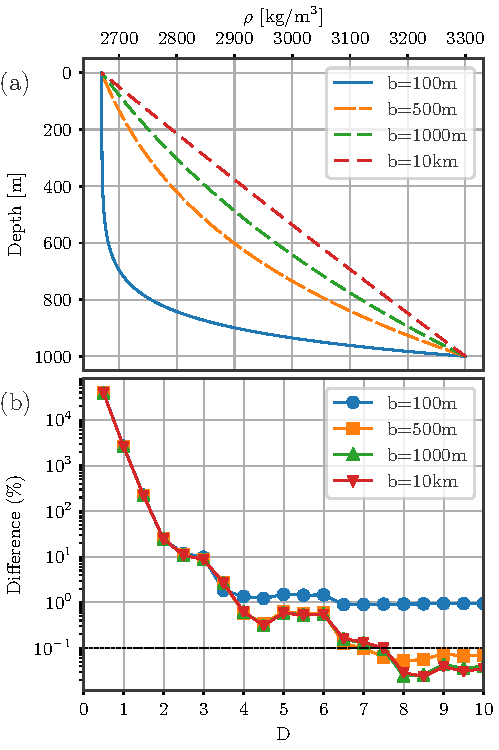
\includegraphics[width=0.9\linewidth]{figures/exponential-b-thin.pdf}
\caption{
    Results of the distance-size ratio determination for different exponential density functions in case of a spherical shell of 1km of thickness.
    (a) Density functions used in the tests, each one with a different value of $b$.
    (b) Differences between the Marussi tensor component $g_{zz}$ generated by the numerical model and the analytical solution for each density function. Each computation was performed on the big grid described in Table \ref{tab:grids}, for different values of the distance-size ratio $D$. If the difference is less than 0.1\%, we consider that the model has achieved an acceptable accuracy.
}
\label{fig:D-exp-power-thin}
\end{figure}

\subsection{Discontinuous Density}

As a final case, we performed the same test with a discontinuous density function:

\begin{equation}
    \rho(r') = 
    \begin{cases}
        \rho_A & \text{if} \, R_1 \leq r' < R_c \\
        \rho_B & \text{if} \, R_c \leq r' \leq R_2 \\
    \end{cases}
\label{eq:density-discontinuous}
\end{equation}

\noindent where $\rho_A$ and $\rho_B$ are constant densities, $R_1$ and $R_2$ are the inner and outer radii of the shell, respectively, and $R_c$ is the radius on which the density change takes place.

The analytical solution for this kind of density is a linear combination of two homogeneous shells with densities $\rho_A$ and $\rho_B$:

\begin{equation}
    V(r) = \frac{4}{3} \frac{\pi G}{r}
    \left[ \rho_A (R_c^3 - R_1^3) +
    \rho_B (R_2^3 - R_c^3) \right]
\end{equation}

Lets assume that $R_c = (R_1 + R_2)/3$ and perform the test for a thin shell of 1km of thickness without applying the density-based discretization algorithm.
Its results can be seen in Figure \ref{fig:D-discont-asym}: up to $D=10$ the difference between the numerical model and the analytical solution is greater than 10\%, what leads us to conclude that a density-based discretization algorithm is needed in order to guarantee the accuracy of the model.

\begin{figure}
\centering
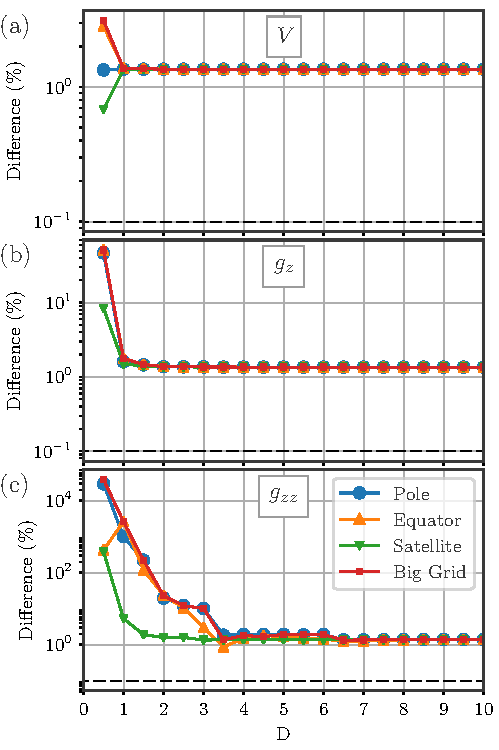
\includegraphics[width=0.9\linewidth]{figures/discontinuous-D-asym.pdf}
\caption{
    Differences between the gravity fields generated by the numerical model and the analytical solution for a thin spherical shell of 1km of thickness with the discontinuous density defined on equation \ref{eq:density-discontinuous}. The computations were performed on the four grids described in Table \ref{tab:grids} and for different values of the distance-size ratio $D$. If the difference is less than 0.1\%, we consider that the model has achieved an acceptable accuracy for the corresponding value of $D$.
}
\label{fig:D-discont-asym}
\end{figure}


%%%%%%%%%%%%%%%%%%%%%%%%%%%%%%%%%%%%%%%%%%%%%%%%%%%%%%%%%%%%%%%%%%%%%%%%%%%%%%%

\section{Determination of delta ratio}

In the light of the previous results, a density-based discretization algorithm is needed in order to achieve an acceptable accuracy in those cases on which the modified adaptive discretization algorithm is not sufficient to take into account the numerical error due to density variations.

Besides the implementation of this new algorithm, we must determine the maximum value of the delta ratio $\delta$ that produces an accuracy bellow a predefined threshold in order to guarantee the good performance of the numerical model.

To do this we applied a similar methodology used in the determination of the distance-size ratio $D$.
Using different values of $\delta$, ranging from 0.1 to 1 with a step of 0.1, we computed the potential, the $g_z$ component of the gradient and the $g_{zz}$ component of the Marussi tensor generated by a spherical shell with several exponential densities (like the one in equation \ref{eq:density-exp}): each one with a different value of $b$.
We performed this tests for a thin and a thick spherical shell of 1km and 35km of thickness, respectively.

Figures \ref{fig:exponential-delta-thin}a and \ref{fig:exponential-delta-thick}a show the exponential density functions used on each test for a thin and thick spherical shell, respectively.
While on Figures \ref{fig:exponential-delta-thin}b and \ref{fig:exponential-delta-thin}b we can see the differences between the resulting $g_{zz}$ with the corresponding analytical solution.
The results for the other gravity fields were excluded from the figures due to their similarities with the ones for $g_{zz}$.

\begin{figure}
\centering
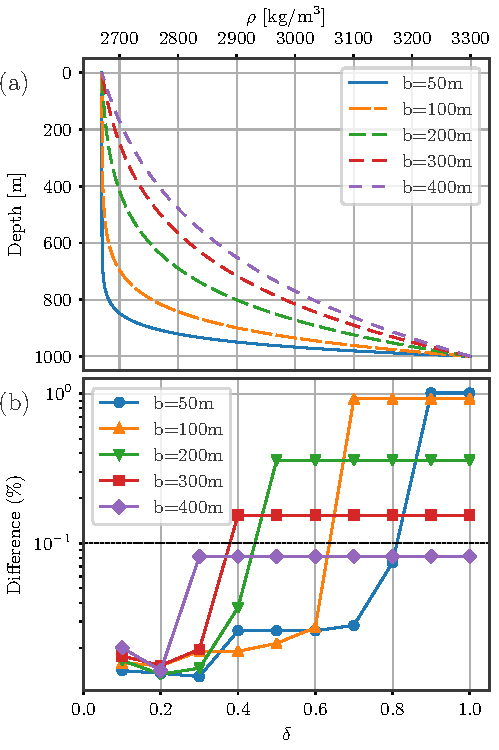
\includegraphics[width=0.9\linewidth]{figures/exponential-delta-thin.pdf}
\caption{
    Results of the delta ratio determination, applied to a thin spherical shell (1km of thickness) with various exponential density functions, each one with different value of $b$.
    (a) Density functions used to perform the test.
    (b) Differences between the $g_{zz}$ component of the Marussi tensor generated by the numerical model and its corresponding analytical solution for several values of $\delta$ and $b$.}
\label{fig:exponential-delta-thin}
\end{figure}

\begin{figure}
\centering
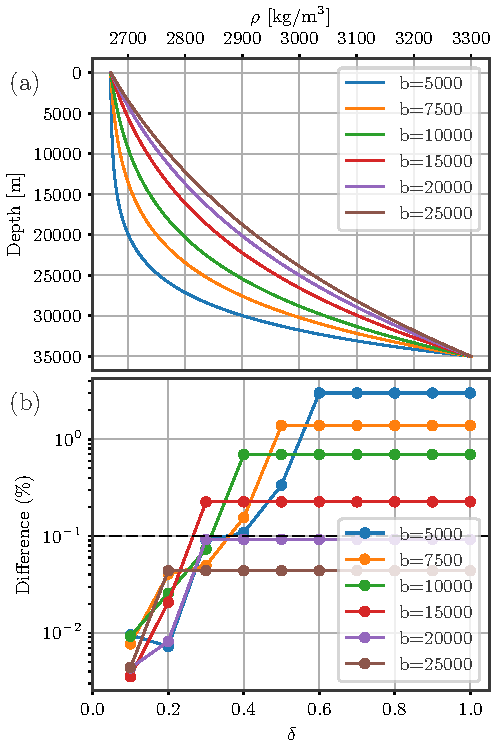
\includegraphics[width=0.9\linewidth]{figures/exponential-delta-thick.pdf}
\caption{
    Results of the delta ratio determination, applied to a thick spherical shell (35km of thickness) with various exponential density functions, each one with different value of $b$.
    (a) Density functions used to perform the test.
    (b) Differences between the $g_{zz}$ component of the Marussi tensor generated by the numerical model and its corresponding analytical solution for several values of $\delta$ and $b$.}
\label{fig:exponential-delta-thick}
\end{figure}

In the thin shell case we can conclude that a delta equal to 0.3 guarantees an acceptable accuracy under 0.1\% for the entire set of the density functions, while the thick shell case needs at least a delta equal to 0.2.
We will keep the more conservative value of 0.2 as the default value of delta on future computations.

Furthermore, we computed the difference between the numerical model and the analytical solution in case of a discontinuous density (as the one in equation \ref{eq:density-discontinuous} with $R_c = (R_1 + R_2)/3$) using a $\delta = 0.2$.
The result for the $g_{zz}$ component of the Marussi tensor is bellow the 0.1\% threshold, achieving a good performance for this default value of $\delta$.


%%%%%%%%%%%%%%%%%%%%%%%%%%%%%%%%%%%%%%%%%%%%%%%%%%%%%%%%%%%%%%%%%%%%%%%%%%%%%%%

\section{Speed Comparison}

We have recorded the computation times for the gravity potential, the gradient component $g_z$ and the Marussi tensor component $g_{zz}$ generated by a single tesseroid model ($35$km of thickness) with homogeneous, linear and exponential density (with $b=50$km) at different heights. Then we calculated the ratio between these computation times:

\begin{equation}
    \text{Computation Times Ratio} =
        \frac{\Delta t_\text{variable}}{\Delta t_\text{homogeneous}},
    \label{eq:computation-times-ratio}
\end{equation}

\noindent where $\Delta t_\text{homogeneous}$ and $\Delta t_\text{variable}$ are the computation times corresponding to the homogeneous model and to the variable density ones (linear and exponential).

On Figures \ref{fig:speed-comparison}a and \ref{fig:speed-comparison}b we can see the results of these comparison.
In the linear density case the density-based discretization algorithm is not applied because the inequation \ref{eq:delta-density} is never satisfied.
For this reason, the homogeneous density model is up to 5 times faster than the variable density one in this case.
On the other hand, the density-based discretization algorithm makes the computation slower: up to 20 times slower than the homogeneous density code.
Nevertheless, this increase in the computation time pays off with a guarantee\todo[inline]{guarantee is a noun?} on its accuracy.

\begin{figure}
\centering
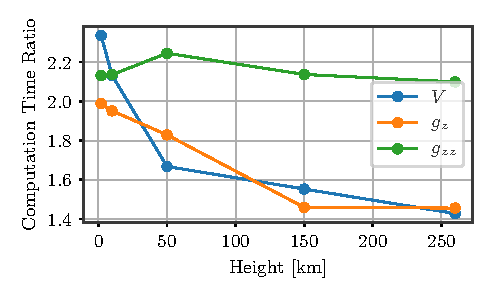
\includegraphics[width=0.9\linewidth]{figures/speed-comparison.pdf}
\caption{Computation time ratio between a single tesseroid model with variable and with homogeneous density at different heights (defined in equation \ref{eq:computation-times-ratio}) for (a) a linear and (b) an exponential density.}
\label{fig:speed-comparison}
\end{figure}


%%%%%%%%%%%%%%%%%%%%%%%%%%%%%%%%%%%%%%%%%%%%%%%%%%%%%%%%%%%%%%%%%%%%%%%%%%%%%%%

\section{Example with real data}

Besides all the tests we have carried out on the new code, we intend to show a forward modelling example with real data.
In order to do that we have chosen the Neuqu\'en Basin: a sedimentary basin located to the east of the Andes, between 32$^\circ$S and 40$^\circ$S latitude (see Figure \ref{fig:neuquen-basin}a), that includes continental and marine siliciclastics, carbonates and evaporites accumulated over the Jurassic and the Cretaceous constituting a stratigraphic record up to 5000m of depth \citep{Howell2005}.

\begin{figure*}
\centering
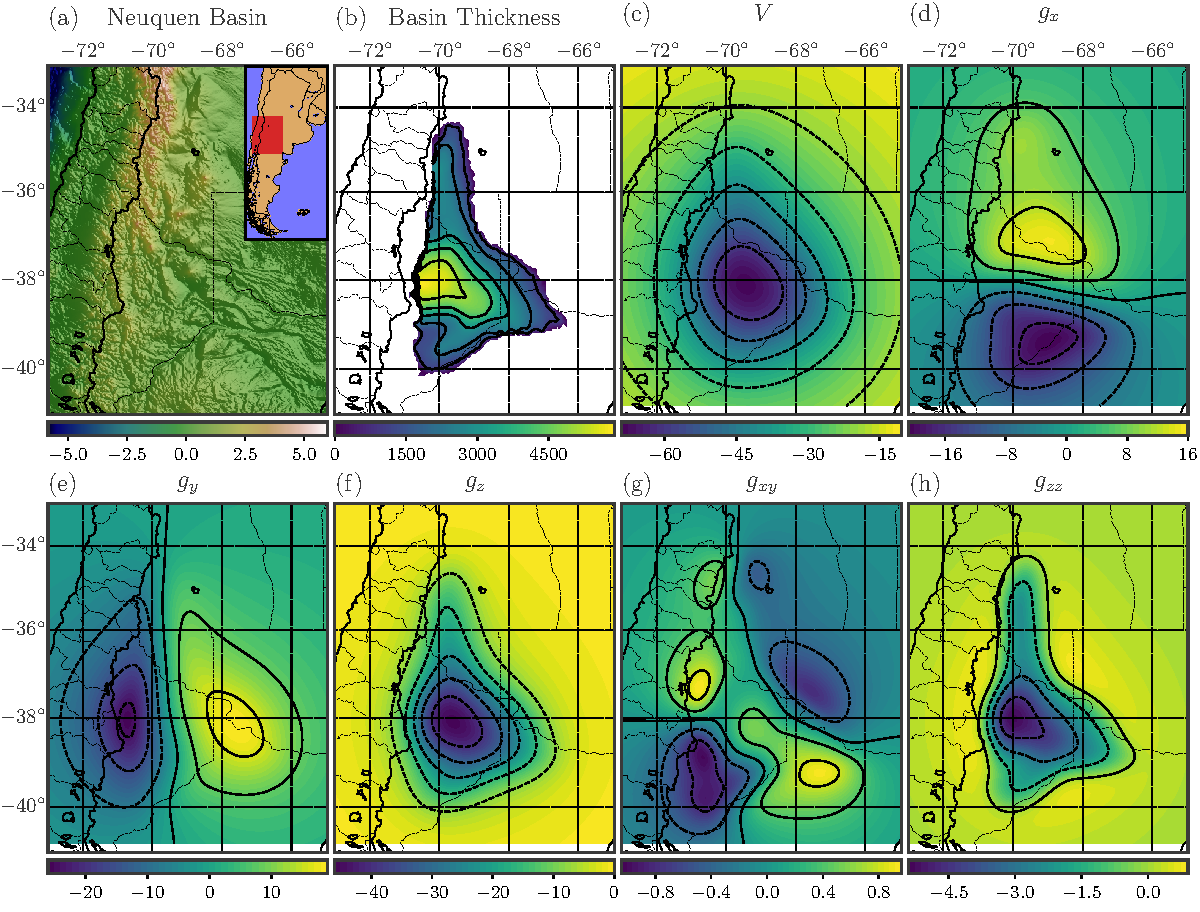
\includegraphics[width=\linewidth]{figures/neuquen-basin.pdf}
\caption{
         Forward model example with real data: Nequ\'en sedimentary modelled through tesseroids with exponential density.
         (a) Topography of Neuqu\'en Basin (in km),
         (b) Thickness of the sedimentary basin (in meters),
         (c)-(h) Computed gravity fields: potential $V$ (in J/kg), gradient components $g_x$, $g_y$ and $g_z$ (in mGal) and Marussi tensor components $g_{xy}$ and $g_{zz}$ (in Eötvös), calculated at 50km of height over the ellipsoid.}
\label{fig:neuquen-basin}
\end{figure*}

The thickness of the sediment pack was obtained from \citet{Heine2007}.
We managed to produce a regular grid with a resolution of 0.05$^\circ$ on both longitude and latitude directions with one value of thickness on each node (see Figure \ref{fig:neuquen-basin}b).

In order to compute the gravity fields generated by this basin we created a mesh of tesseroids, each one located on one of the nodes of the grid, with dimensions of 0.05$^\circ$ $\times$ 0.05$^\circ$ and depth equal to the thickness of the basin on the corresponding node.

We must also define a density function for the entire model.
\citet{Sigismondi2012} proposed a minimum and maximum density contrast for the Neuqu\'en basin of -412kg/m$^3$ and -275kg/m$^3$, respectively. \todo[inline]{ver que esos valores son de contraste y tienen q ir negativos. poner los valores absolutos.}
So we have chosen, for this specific example, an exponential density (like the one in equation \ref{eq:density-exp}) that assumes the minimum value on the surface and the maximum at 5858m, i.e. the bottom of the basin, with a value of $b$ equal to 3km.

We have finally computed the gravity potential $V$, the gradient components $g_x$, $g_y$ and $g_z$, and the Marussi tensor components $g_{xy}$ and $g_{zz}$ on a computation grid of 159$\times$163 nodes with a 0.05$^\circ$ spacing on both longitude and latitude directions at a 50km height over the reference ellipsoid.
The resulting gravity fields can be seen in Figures \ref{fig:neuquen-basin}c-h.
We have excluded the other components of the Marussi tensor from the Figure, although they can be found in the repository.


%%%%%%%%%%%%%%%%%%%%%%%%%%%%%%%%%%%%%%%%%%%%%%%%%%%%%%%%%%%%%%%%%%%%%%%%%%%%%%%

\section{Conclusions}

We have developed a Python library that allows us to perform forward gravity computations using tesseroids with variable density in depth.
The code numerically approximates the integral that defines the gravity potential, its gradient and the Marussi tensor through the Gauss-Legendre Quadrature (GLQ).
It essentially consists in approximating the gravity fields of the tesseroids with the effect of point masses located on the scaled nodes of the Legendre polynomials.
We state that this method it's well suited to approximate the effect of tesseroids with arbitrary densities, in contrast with the ones that involve Taylor series expansion.

Instead of enhancing the accuracy of the method by increasing the order of the GLQ on each integration, we make use of the preexisting modified adaptive discretization algorithm and a new density-based discretization algodithm.

The former one divides the tesseroid by half if the ratio of the distance to the computation point and its size is lower than a predefined distance-size ratio $D$.
We can summarise that $D$ controls the accuracy of the method: a higher value of $D$ generates more divisions of the tesseroids, thus more point masses, what leads to a more precise approximation.
Nevertheless it is not sufficient to guarantee the accuracy of the method in case of specific density functions as a highly variable exponential or some discontinuous functions.

For this reason we developed a density-based discretization algorithm that divides the tesseroid on the radius at which the \emph{maximum variation} of the density function takes place, only if a certain inequation that relates this \emph{maximum variation} with a predefined delta ratio $\delta$ holds.
Therefore the number of subdivisions is indirectly controlled by this delta ratio $\delta$, and thus the accuracy of the computation.

Because there is no direct relation between the values assigned to $D$ and $\delta$ and the error of the computation, we had to empirically determine the minimum value of $D$ and the maximum value of $\delta$ that produce an acceptable accuracy for each gravity field.

The distance-size ratio determinations have been made through the comparison of the numerical approximations with the analytical solutions for a spherical shell with variable density, which had to be analytically obtained.
These tests have been made without applying the density-based discretization algorithm in order to isolate the former one.
From the wide range of possible density variations, we've chosen a linear, an exponential and a discontinuous density functions.
The comparisons over the first two functions have shown that values of $D$ equal to 1, 2 and 8 for the calculation of the gravity potential, its gradient and the Marussi tensor components, respectively, produce an accuracy of 0.1\% or better.
On the other hand, the algorithm on its own does not guarantee this amount of accuracy in case of highly varying exponential functions or discontinuous densities.

We have performed similar tests for the density-based discretization algorithm comparing the numerical model with the analytical solutions for a spherical shell with various exponential densities: from low to high varying functions.
Each comparison was made for different values of $\delta$, keeping the default values of $D$ previously obtained.
This tests have shown that a value of $\delta = 0.2$ guarantees an accuracy of 0.1\% or better on every case, while the same results can be obtained performing this tests with the discontinuous density function.
The default value $\delta$ is the same for every gravity field computation.

Moreover, we had performed speed comparisons between tesseroids models with homogeneous and variable densities, showing that a high varying density function requires more computation time than a low varying one, as expected.

Finally, we have shown a real data example: we have computed the gravity fields generated by the Neuqu\'en sedimentary basin through a tesseroid model with exponential density with depth on a regular grid at 50km height.


%%%%%%%%%%%%%%%%%%%%%%%%%%%%%%%%%%%%%%%%%%%%%%%%%%%%%%%%%%%%%%%%%%%%%%%%%%%%%%%

\section{Acknowledgments}

We are indebted to the developers and maintainers of the open-source
software without which this work would not have been possible.

%%%%%%%%%%%%%%%%%%%%%%%%%%%%%%%%%%%%%%%%%%%%%%%%%%%%%%%%%%%%%%%%%%%%%%%%%%%%%%%

\bibliographystyle{gji}
\bibliography{references}

\end{document}
